\documentclass[a4paper,titlepage]{article}
\usepackage{frontespizio}
\usepackage[english]{babel}
\usepackage[utf8]{inputenc}

\usepackage[a4paper, total={6in, 9in}]{geometry}
\usepackage{rotating}


\begin{document}
\begin{frontespizio}
\Universita{Verona}
\Dipartimento{Informatica}
\Corso[Laurea]{Informatica}
\Titoletto{Software Engineering}
\Titolo{Second project report}

\Candidato[VR363021]{Giovanni Liboni}
\Candidato[VR359169]{Enrico Giordano}
\Candidato[VR359129]{Alberto Marini}
\Candidato[VR359333]{Alessandro Falda}

\Annoaccademico{2013-2014}
\end{frontespizio}

\tableofcontents

\newpage

\part{Introduction}

This project implements an asynchronous system and consists in three principal parts:

\begin{enumerate}

\item a station, that controls speed of cars;

\item some automatic cars, that set their velocity randomly during the ride and gain the ideal velocity thanks to the station;

\item some manual cars, that set their velocity randomly during the ride and receive ``break'' message (but they are not obliged to slow down).

\end{enumerate}

During the execution, 50 manual cars and 40 automatic cars are instantiated; during the runtime their speeds changes randomly. After a simple ride, the cars decide randomly if they will exit or not. 

\newpage

\part{Graphical interface}

The graphical interface is built with \textit{swing} Java library and consists of two JFrame called ``WallGraphic'' and ``DebugInterface''. The first interface (WallGraphic) is a representation of the situation, composed by a station, some automatic cars and some manual cars. The second interface (DebugInterface) is a textual console that shows the program flow, cars' display and state and station state. This interface has three option:

\begin{figure}[!h]
\centering
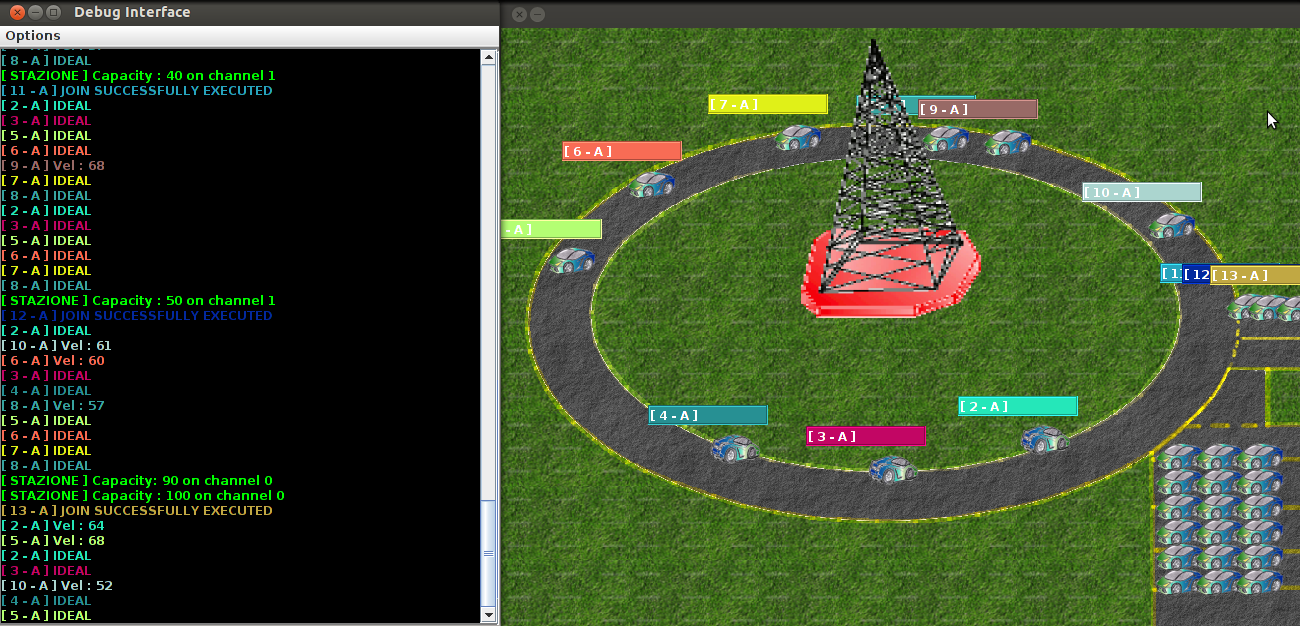
\includegraphics[scale=0.3]{screen.png}
\caption{ScreenShot}
\end{figure}

\begin {enumerate}

\item ``pause'', that stops the program's flow acquisition;

\item ``resume'', that resume the program's flow acquisition (and enable autoscroll);

\item ``watch'', that disables or enables the autoscroll of the scrollbar.    

\end{enumerate}


The DebugInterface is composed by a JFrame that contains a JPanel that contains a JTextArea with a black background and a text that is updated by both the station and the cars' displays.

~

WallGraphic is composed by a JFrame that contains a JPanel with a ``wallpaper'' (the circuit). This JPanel contains in different levels (Z ordered) a station (that is a JLabel with an image) and some cars (that are JLabels with an image). The cars move in asynchronous way into the ride in 10 different direction (in order to approximate the elliptical path).

On the car label there is a Jlabel showing its id and car type: the ``M'' letter represent the ``Manual car'' and the ``A'' letter represent the ``Automatic car''. When a car change its direction (X orientation), its image changes.

\begin{figure}[!ht]
\centering
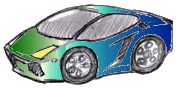
\includegraphics[scale=0.2]{../car.png}
\caption{car label}
\end{figure}


\begin{figure}[!ht]
\centering
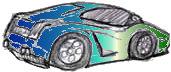
\includegraphics[scale=0.2]{../car2.png}
\caption{car label (different orientation)}
\end{figure}

\begin{figure}[!ht]
\centering
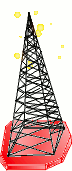
\includegraphics[scale=0.5]{../radio.png}
\caption{station label}
\end{figure}


Every car is a graphical thread that execute the move() method in order to change the position forward the ride; when a car exits the circuit, the thread dies. The speed is represented graphically by a thread sleep during the movement.

~

This is the Z order of the JLabel:

~

~ ~ ~ ~ ~-1: background image;

~

~ ~ ~ ~ ~ 0: station;

~

~ ~ ~ ~ ~ 1: cars;

~

In this way, the cars will pass graphically behind the station and on the background image.


In the park, there are a lot of ``dead cars'' that simply stand still in there. This was made to fill a space that could seem empty or messy.

~

The graphical classes are contained in the \textit{``graphics''} package.

\section{Design pattern for graphical interface}

Every class of this project must use these graphical interface, so a \textbf{Façade pattern} was implemented. In fact there is a general class, ``ScenarioGraphic'', including every graphical instance; in this way, when a class needs to use a graphical instance, it simply calls the ScenarioGraphic methods and ScenarioGraphic can modify the graphical istances. 
\newpage
\begin{figure}[!ht]
\centering
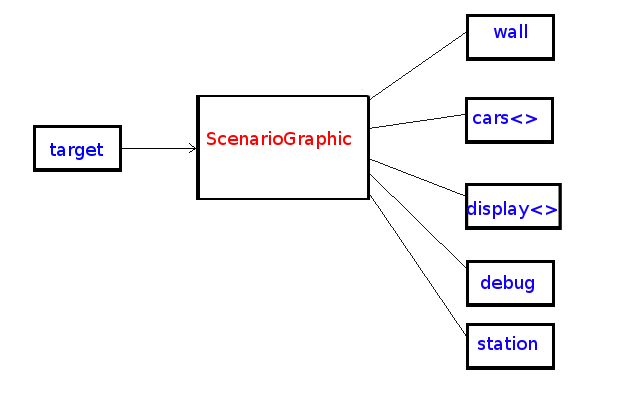
\includegraphics[scale=0.4]{facade.png}
\caption{Façade pattern}
\end{figure}

\newpage

\section{Swing bug}

The Swing graphical library is a simple and useful library for java applications, but in this project it was used at the limit of its potential. So, every car has two graphic threads that work asynchronously with a fast refresh (20 milliseconds). During the execution the GUI could show this exception: 

\begin{verbatim}
Exception in thread "Thread-1" java.lang.NullPointerException
	at javax.swing.BufferStrategyPaintManager.flushAccumulatedRegion
	...
\end{verbatim}

This is a bug of Swing library dealing with the management of asynchronous threads that have a very high refresh. Anyway it is not important for the program's execution, given its rare occurrence.

\newpage

\part{AutoCar and ManCar Classes}

%Queste classi sono delle implementazioni delle interfacce di tipo Runnable e InterfaceAutoCar (e il rispettivo InterfaceManCar) per questi motivi: 
These classes are implementations of Runnable and InterfaceAutoCar interfaces (and the respective InterfaceManCar) for these reason:

\begin {itemize}

\item they contain a method \begin{verbatim} public void run() \end{verbatim} which represents the mouvement of each car (i.e. run the route in the circuit);
%\item contengono un metodo \begin{verbatim} public void run() \end{verbatim} che rappresenta ciò che ogni macchina deve fare dal punto di vista del movimento (cioè eseguire il tragitto nel circuito);

%\item implementano le corrispettive classi della loro interfaccia.
\item they implement the corresponding classes of their interface.

\end {itemize}

%Il fatto di implementare due interfacce differenti è stato utile per rappresentare un comportamento diverso come da specifiche per il messaggio di ``break'' ricevuto dalla stazione e in particolar modo per utilizzare il design pattern di tipo \textbf{Adapter}. Infatti avendo due implementazioni differenti, per utilizzare diversamente un metodo non è possibile fare un Override e quindi bisogna appoggiarsi ad una classe intermedia (AdapterAutoToManual) che estende la classe chiamante ma implementa la classe da cui si vuole ereditare il comportamento.   
Implementing two  different interfaces is useful in order to represent a different behavior for the ``break'' message received from the station and in particular for using \textbf{Adapter} design patterns type. In fact, to use a different method you cannot make an override and so you have to rely on an intermediate class (called AdapterAutoToManual) that extends the calling class but implements the class which from which you want to inherit the behavior.

%Quindi di fatto esistono due interfacce distinte di AutoCar e ManCar che vengono implementate dalle rispettive classi e che hanno comportamenti differenti; se si vuole utilizzare la AutoCar come ManCar bisogna istanziare la classe AdapterAutoToManual e utilizzare tramite essa i metodi della classe ManCar. 
So in fact there are two distinct interfaces to AutoCar and Mancar that are implemented by the respective classes and have different behaviors; if you want to use the AutoCar as a ManCar you must instantiate the AdapterAutoToManual class and use through it the ManCar class methods.

\begin{figure}[!ht]
\centering
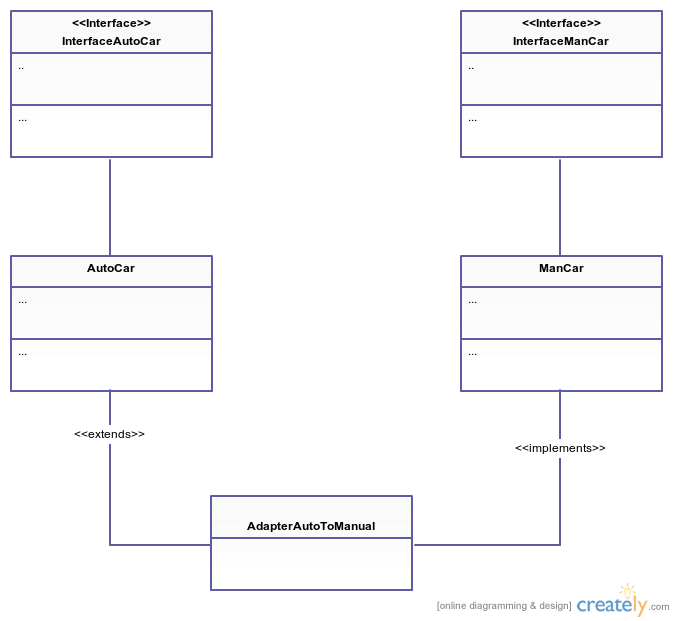
\includegraphics[scale=0.4]{adapter.png}
\caption{Adapter pattern}
\end{figure}


\newpage

%Per rendere possibile l'utilizzo della propria parte grafica da parte della classe AutoCar e ManCar, è stato fatto in modo che questa classe istanziasse dentro di essa l' istanza grafica ``CarGraphic'', in modo da avere pieno controllo sulla propria parte grafica. 
To make possible the use of graphics part by AutoCar and ManCar classes, this class can instantiate in it the ``CarGraphic'' graphics instance, in order to have full control over their graphics part.

%Questo è stato utile per gestire il movimento delle macchine in maniera asincrona rispetto alle altre macchine ma anche all'esecuzione del programma. Inoltre in questo modo anche alla classe ScenarioGraphic è permesso di avere controllo del comportamento e della parte grafica sia delle AutoCar sia delle ManCar; istanziando infatti la classe AutoCar o ManCar, si crea in automatico l'istanza grafica, quindi è possibile gestirla facendo accesso alle singole istanze delle loro classi. 
This was useful for managing the asynchronously car movements compared the other cars, and for the execution of the program too. Moreover, in this way ScenarioGraphic is allowed to have control of behavior and the graphical parts of both AutoCar and Mancar classes; in fact, by instantiating Mancar or AutoCar class it automatically creates the graphic instance, so you can manage it by accessing the individual instances of their classes.

~

%Questo rende inoltre utile l'utilizzo del \textbf{Façade Pattern}, perché si vuole utilizzare una singola classe per controllare tutte le istanze grafiche (dove è permesso).
As a consequence the use of \textbf{Facade Pattern} is useful, because you can use a single class to control all graphical instances (where permitted)

\newpage

\part{Communication}

The communication is based on two main components: the network (called Net) and the communication module (called Comunication). The network stores the cars within the range of action and within the circuit. The communication manages the exchange of messages, in receiving and in transmission, and notifies to the upper component the receiving of a message.

~

The project specified a limitation of the available band of a station to receive and a limitation of number of car to send. This problem has been simulated using the sleep() method, so we send and receive only the predetermined number of times.
During the sleep period, the car can receive messages, thanks to a tail that serves as a buffer. When the car receives a message, the module
notifies that to the car using the update() method.

~

The station receives the messages, stores them into a vector that serves as a buffer and then, when the principal thread wakes up, the station download the vector. So, the received packets are passed to the station to be processed.
The station uses a broadcast method to send to all the cars into the circuit the same packet.
A package is composed by two objects: the sender's ID and the messages. Every message is composed of the data and the recipient. In this way, you minimize the number of packets sent from the station and you can send more broadcasted messages simultaneously, in order to get faster feedback by cars.

~

The communication part has been specialized depending on whether the component was a station or a car. The car module will send messages at a rate defined by ts pps; on the other side, the station hasn't this limitation. 
The network's operation can be grouped into stages: the entry into the field of action of the network by a car, the join request from the station, the station response, the entry in the circuit and the exit from the circuit.

~

When a car enters into the field of action of the station and its network, the station sends a broadcast message to all cars with a JOIN message. This message will be ignored by the cars already in the circuit and will be managed by the cars into the parking and the cars just entered in the field. When a car receives a station ok to get in, it enters into the circuit and starts sending the data of its speed at the station. When the car must leave the circuit, the car is removed from the cars inside the circuit and inside the range of network.

~

If a car does not receive the station OK, it goes into the park and it waits a free place into the network.
The parking is managed with a FIFO queue, to comply the order of entry into the field.
The station sends a broadcast message when a car enters into the field or if there are cars into the parking.

~

The station manages the received packets from the cars and for each message into the packet responds with an IDEAL message, if the car is going at the right speed, otherwise responds with a BREAK message, if the car is going too fast.
It also manages the JOIN request by the cars, by checking if is possible to add them into the network, and, if so, by sending an OK message. In the event that there was no place available, the station sends a BUSY message, denying access to the circuit.
The speed of message receiving is simulated by a sleep, calibrated to receive packets 20 times per second. Every time the station reads the messages from the Comunication module, moves all messages in a internal vector and manages them all at once.

\newpage
\part{UML Class Diagram}


\begin{sidewaysfigure}[!ht]
\centering
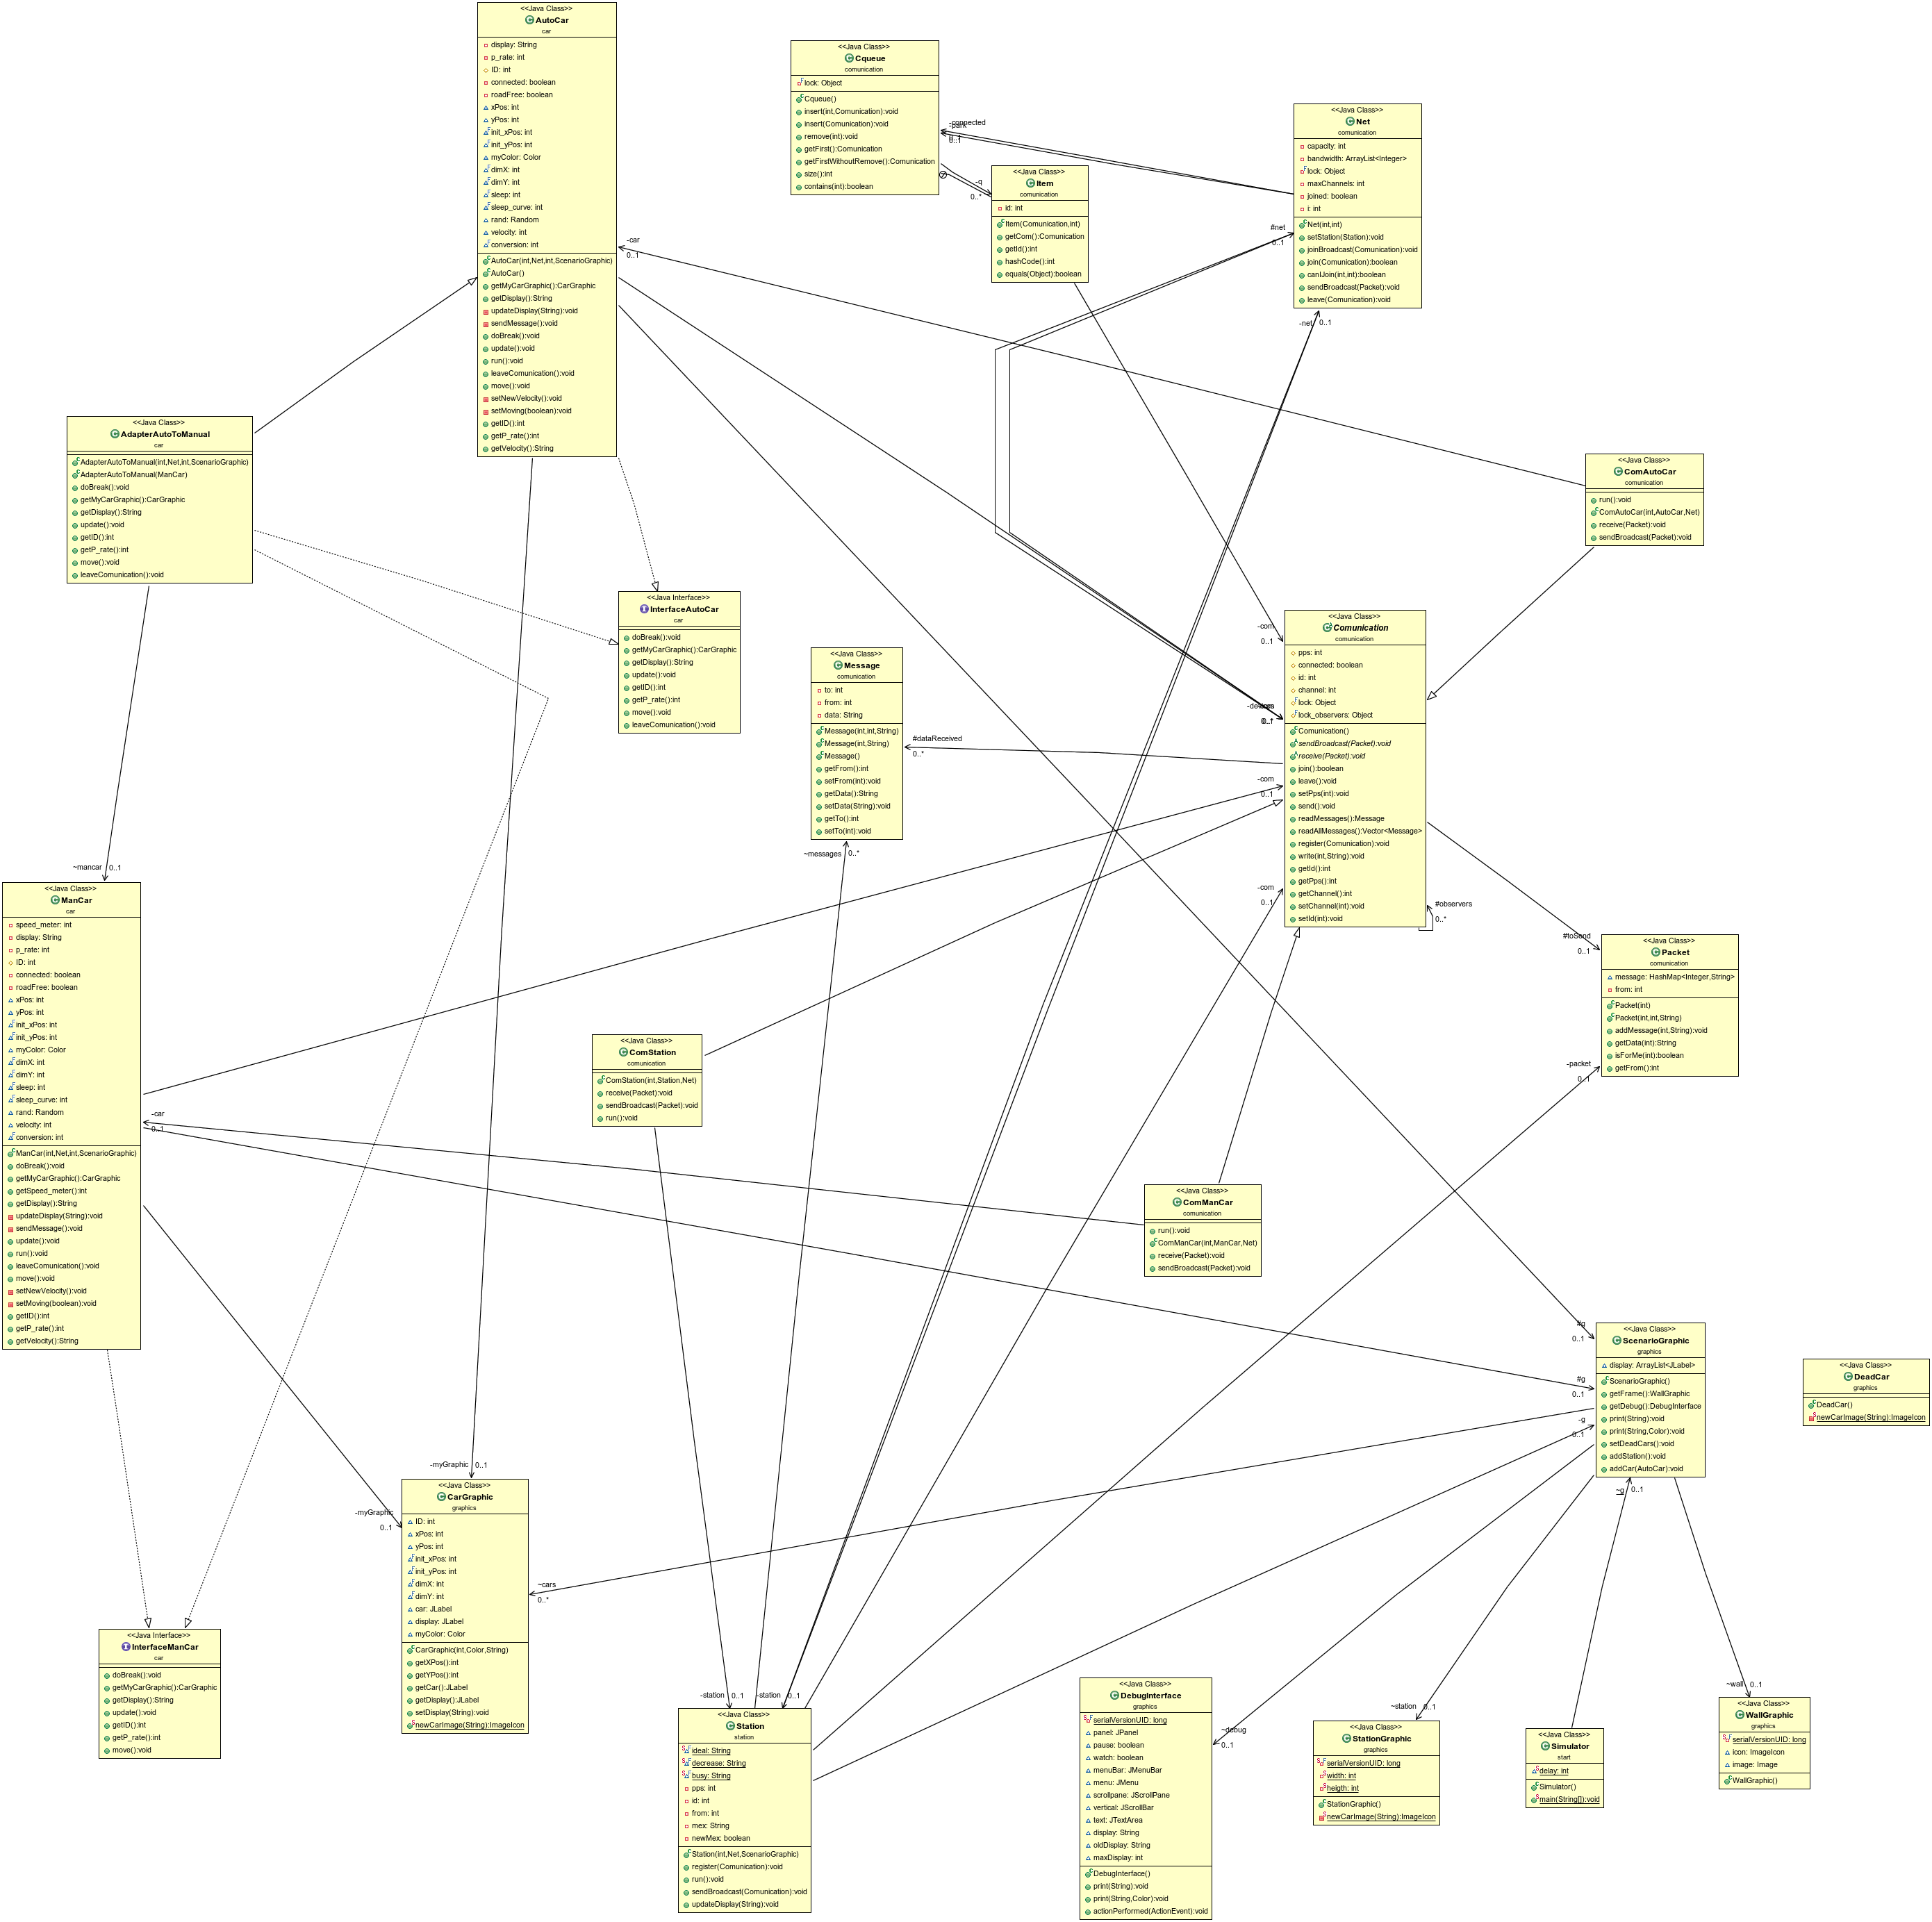
\includegraphics[scale=0.2]{classDiagram.png}
\end{sidewaysfigure}


\end{document}
